% HMC Math dept HW template example
% v0.04 by Eric J. Malm, 10 Mar 2005
\documentclass[12pt,letterpaper,boxed,cm]{hmcpset}

% set 1-inch margins in the document
\usepackage[margin=1in]{geometry}
\usepackage{mathtools}
\usepackage{mathrsfs}
% include this if you want to import graphics files with /includegraphics
\usepackage{graphicx}
\usepackage{cases}
\usepackage{hyperref}
\usepackage{siunitx}
\usepackage{tikz}
\usepackage{cases}
\usetikzlibrary{arrows}

% info for header block in upper right hand corner
\name{Name: ~~~~~~~~~~~~~~~~~~~~~~~~~~~~}
\class{Physics 51}
\assignment{Homework \#11}
\duedate{October 10, 2016}

\newcommand{\ev}[2]{\Big|_{#1}^{#2}}
\newcommand{\evv}[2]{\Big|_{#1}^{#2}}
\newcommand{\set}[1]{\left\{#1\right\}}
\newcommand{\s}[1]{\sqrt{#1}}
\newcommand{\f}[2]{\frac{#1}{#2}}
\newcommand{\p}[2]{\frac{\partial #1}{\partial #2}}
\providecommand{\t}[1]{\text{#1}}
\providecommand{\span}[1]{\text{span}\left(#1\right)}
\providecommand{\set}[1]{\left\{#1\right\}}
\providecommand{\l}[0]{\left}
\providecommand{\r}[0]{\right}
\newcommand{\m}[1]{\begin{matrix}#1\end{matrix}}
\newcommand{\bm}[1]{\begin{bmatrix}#1\end{bmatrix}}
\renewcommand{\bf}[1]{\mathbf{#1}}
\newcommand{\pn}[1]{\left( #1 \right)}
\newcommand{\abs}[1]{\left| #1 \right|}
\newcommand{\bk}[1]{\left[ #1 \right]}
\newcommand{\cis}[1]{\pn{\cos\pn{#1} + i\sin\pn{#1}}}
\newcommand{\cisi}[1]{\pn{\cos\pn{#1} - i\sin\pn{#1}}}
\renewcommand{\Im}[1]{\text{Im}\pn{#1}}
\renewcommand{\Re}[1]{\text{Re}\pn{#1}}
\renewcommand{\k}[0]{\f{1}{4\pi\epsilon_0}}
\renewcommand{\part}[1]{\vspace{1em}\noindent(#1)}

\makeatletter
\renewcommand*\env@matrix[1][*\c@MaxMatrixCols c]{%
  \hskip -\arraycolsep
  \let\@ifnextchar\new@ifnextchar
  \array{#1}}
\makeatother
\begin{document}
\problemlist{33-P8*, 33-E33, 10, SUP19}

\begin{problem}[33-P8]
	Figure 33-53 shows a cross section of a long conductor of a type called a coaxial cable of radii $a$, $b$, and $c$. Equal but antiparallel, uniformly distributed currents $i$ exist in the two conductors. Derive expressions for $B(r)$ in the ranges
	\begin{enumerate}
		\item[(a)] $r < c$, 
		\item[(b)] $c < r < b$, 
		\item[(c)] $b < r < a$,  and
		\item[(d)] $r > a$.
		\item[(e)] Test these expressions for all the special cases that occur to you.
		\item[(f)] Assume that $a = \SI{2.0}{cm}$, $b = \SI{1.8}{cm}$, $c = \SI{0.40}{cm}$, and $i = \SI{120}{A}$ and plot $B(r)$ over the range $0 < r < \SI{3}{cm}$.
	\end{enumerate}
	\begin{center}
		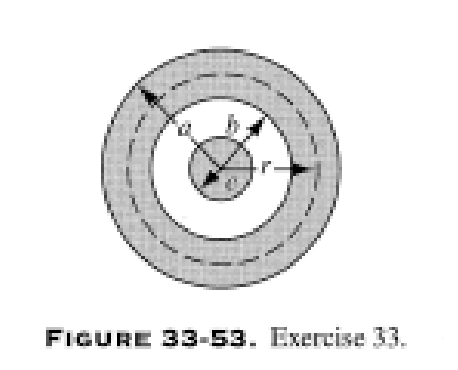
\includegraphics[scale=0.7]{01.png}	
	\end{center}
\end{problem}
\begin{solution}	
\end{solution}
\newpage

\begin{problem}[33-E33]	
Consider an infinite slab of thickness $\mathbf{d}$ carrying a nonuniform current density (current per unit area) $\mathbf{j} = \mathbf{a} |\mathbf{z}|$ along the positive $x$-axis, where the slab is arranged parallel to the $x$-$y$ plane, with the origin in its middle. Find the magnetic field everywhere (HINT: $B$ must be zero on the $x$-$y$ plane; why?).
\end{problem}
\begin{solution}
\end{solution}
\newpage

\begin{problem}[10]	
	In a certain region there is a uniform current density of \SI{15}{A/m^2} in the positive $z$ direction. What is the value of $\oint \vec{\mathbf{B}}\cdot d\vec{\mathbf{s}}$ when the line integral is taken along the three straight-line segments from ($4d$, 0, 0) to ($4d$, $3d$, 0) to (0, 0, 0) to ($4d$, 0, 0), where $d = \SI{23}{cm}$.
\end{problem}
\begin{solution}
\end{solution}
\newpage

\begin{problem}[33-P8*]	
	A thin plastic disk of radius $R$ has a charge $q$ uniformly distributed over its surface. If the disk rotates at an angular frequency $\omega$ about its axis, show that the magnetic field at the center of the disk is
	\[
		B = \f{\mu_0\omega q}{2\pi R}.
	\]
	(Hint: The rotating disk is equivalent to an array of current loops.)
\end{problem}
\begin{solution}
\end{solution}


\end{document}